\begin{doublespace}

\chapter{Experimental evolution of the snowball effect
  shows the importance of complex epistasis in speciation}
\label{chap:snowball}



\section{Introduction}

% Background on the snowball effect

Biological speciation is the evolution of barriers that hinder interbreeding
between populations (`reproductive isolating barriers') \citep{coy04}.
%
Postzygotic barriers cause hybrids between species to be sterile or inviable,
sometimes because genes from different species are incompatible~\citep{coy04}.
%
The Dob\-zhan\-sky-Mul\-ler model of postzygotic isolation (Fig.~\ref{dm-model})
proposes that genetic incompatibilities form as a byproduct of the genetic
divergence between independently evolving populations~\citep{orr95}.
%
The Dob\-zhan\-sky-Mul\-ler model predicts that the number of genetic
incompatibilities, called `Dob\-zhan\-sky-Mul\-ler incompatibilities' (DMIs),
should increase faster than linearly through time~\citep{orr95,orr01}.
%
For example, pairwise DMIs (i.e., DMIs between two alleles)
should increase quadratically through time~\citep{orr01}.
%
This phenomenon has been called the `snowball effect'~\citep{coy04}.



\begin{figure}
\begin{center}
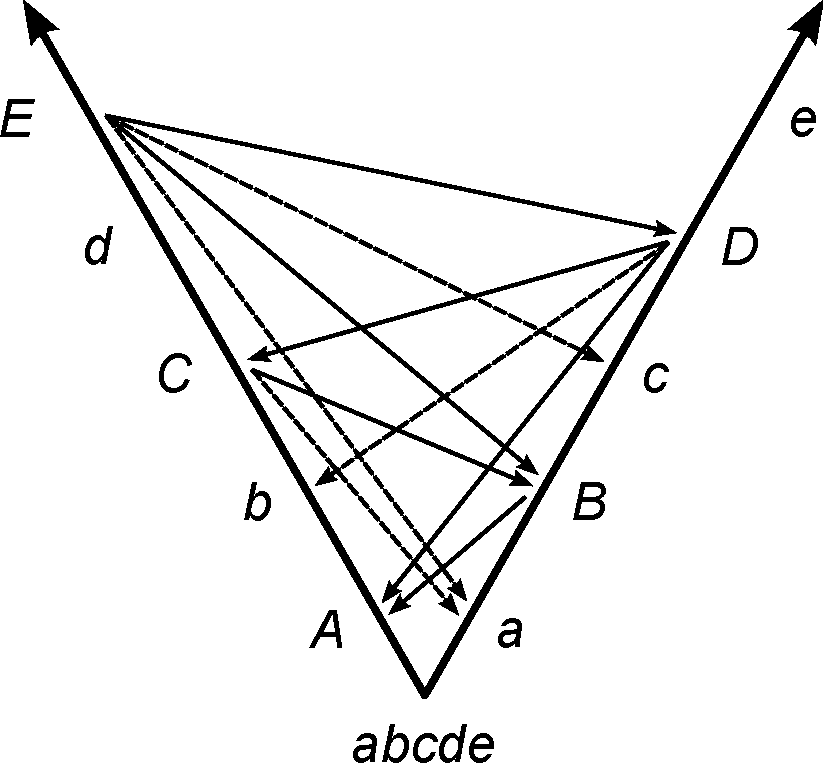
\includegraphics[width=3.5in]{dm-model.pdf}
\end{center}
\caption{\textbf{The Dob\-zhan\-sky-Mul\-ler model of postzygotic isolation.}
%
A population with haploid genotype \emph{abcde} (bottom)
becomes geographically divided into two,
and each population independently evolves through time
(thick arrows, time progresses upward).
%
In the first population,
allele \emph{a} is substituted with allele \emph{A},
while in the second population
allele \emph{b} is substituted with allele \emph{B}.
%
At this point, if the populations were to come into contact and hybridize,
their hybrids would have genotypes
\emph{Abcde}, \emph{aBcde}, or \emph{ABcde}.
%
Because alleles \emph{A} and \emph{B}
evolved independently and thus may only function properly
in the background in which they evolved,
hybrids with genotype \emph{ABcde} may be sterile or inviable.
%
In this case, alleles \emph{A} and \emph{B} are said to form a
Dob\-zhan\-sky-Mul\-ler incompatibility (DMI)
(arrow from \emph{B} to \emph{A}).
%
The populations could have instead hybridized
after two or more alleles have fixed within each lineage
(e.g., alleles \emph{A}, \emph{C}, and \emph{E} in the first population
and alleles \emph{B} and \emph{D} in the second),
which would have resulted in hybrids with many more possible DMIs.
%
DMIs between derived alleles (`derived-derived' DMIs) are thin solid arrows,
and DMIs between derived and ancestral alleles (`derived-ancestral' DMIs)
are thin dashed arrows.
%
(Modified from \citep{orr95}.)}
\label{dm-model}
\end{figure}



% No support for the snowball effect

Several tests of the snowball effect have not supported it
\citep{lij03,men04,gou10}, concluding that there is a `missing snowball.'
%
These tests, however, relied on indirect methods
because testing the snowball effect directly is difficult \citep{men04}.
%
Rather than using a single pair of species and following it through time,
researchers have used different pairs of species diverged at different times
\citep{mal08,sco08}.
%
For the number of DMIs, the strength of postzygotic isolation,
often measured as the reduction in hybrid viability or fertility, has been used.
%
However, for the strength of postzygotic isolation to be a good proxy
for the number of DMIs,
the fitness effects of DMIs on hybrid fitness must be additive
\citep{men04,bol05}
(e.g., twice the number of DMIs should result in twice the isolation),
but whether this is true is not known \citep{bol05,pre10}.



% Support for the snowball effect

Better estimates of the number of DMIs between two species
were recently carried out by two studies \citep{mat10,moy10},
both supporting the snowball effect.
%
To estimate the number of DMIs, they introgressed single genetic regions
of one species into the genetic background of the other and
counted the number of introgressions with reduced viability or fertility.
%
However, this method cannot identify individual DMIs
but rather whether a genetic region of one species
is incompatible with something in the other.
%
As with the previous methods, they relied on the ages of species pairs
rather than following a single species pair through time.
% According to Applied Longitudinal Data Analysis (p. 9), this is bad:
% (http://www.gse.harvard.edu/~faculty/singer/Papers/ch1&2.pdf)
%
In addition, because these studies could only obtain
at most three species pairs with which to count the number of DMIs,
their quadratic fit to the data was not statistically powerful.



% Sample identification of a DMI

To provide an example of what is required to identify a DMI,
suppose that allele $D$ in Fig.~\ref{dm-model} has just fixed
in one population, and I want to test whether it is incompatible
with allele $C$ in the other population.
%
One option is to isolate these alleles in the ancestral genetic background
(\emph{abcde}) to construct the genotype \emph{abCDe} and measure its fitness.
%
In this constructed genotype, however,
alleles $D$ and $b$ as well as alleles $C$ and $a$
may also be incompatible (Fig.~\ref{dm-model}),
and therefore confound the effect of $C$ and $D$ together.
%
Every other possible construction of a genotype that includes $C$ and $D$
(i.e., \emph{aBCDe}, \emph{AbCDe}, and \emph{ABCDe})
also contains other possibly confounding incompatibilities.
%
To prevent these confounding factors, one may only consider
alleles that were compatible with the ancestral background.
%
In the example above, this means that one must first verify that genotypes
\emph{abCde} and \emph{abcDe} had normal fitness before testing \emph{abCDe}.


%- here's what I did
%- here's what I used to do it
%- here's why I used it
%  - accurately count...
%- here's what I got


In this study, I conducted experimental evolution
to test whether pairwise DMIs increased quadratically through time
between evolving populations of digital organisms.
%
I also measured hybrid inviability through time
in order to determine whether there was a missing snowball.
%
Finally, I determined the ratio of derived-derived and derived-ancestral DMIs
and the probability than a pairwise interaction forms a DMI,
which in the literature has been assumed to be constant.
%
I used Avida~\citep{ofr04} (see p. \pageref{sec:avida},
an artificial life research platform,
to conduct our experiments with digital organisms.
%
I used digital organisms for several reasons:
I can observe thousands of generations in minutes,
easily manipulate genomes, which allowed us to
develop a method to accurately count the number of individual pairwise DMIs
as they arose,
and have an accurate historical record.



% I want to end the Introduction with "a brief statement of the overall aim
% of the experiments and a comment about whether that aim was achieved" (PLoS).
% An idea is to move first half of "Science papers" paragraph with
% the paragraph before, then move second half to the end (as a last paragraph)
% and expand more on the results and their significance.

% Need to update fig \ref{avida}B with new epistasis figure (directory try_2)



\section{Results}

To generate the ancestral genotype, I first founded a population
with an organism that could replicate sexually but could not perform any tasks.
%
I then let this population evolve for about 1.5 million generations,
and I took the genotype of the most common organism as the ancestral genotype.
%
Using this ancestor, I then founded 40 independent populations
and allowed them to evolve independently for about 10,000 generations.
%
The configuration parameters, including the environmental conditions,
were the same as those of the ancestor.
%
Every 400 generations, the entire population was saved for later analysis.
%
Because the ancestor was well-adapted to its environment,
the genetic divergence between replicate populations
was mostly due to fixation of neutral mutations.
%
Thus, the rate of substitution for each population
was approximately constant (Fig.~\ref{avida}C),
satisfying an assumption of the snowball effect
when it is analyzed through time \citep{orr95}.
%
The mean relative fitness of hybrids between pairs of populations
at the end of the runs was 0.91 (range: 0.68--0.97) (Fig.~\ref{avida}D),
indicating that incomplete postzygotic isolation had evolved.
%
From now on, I refer to these populations as `species.'



\begin{figure}[p]
\begin{center}
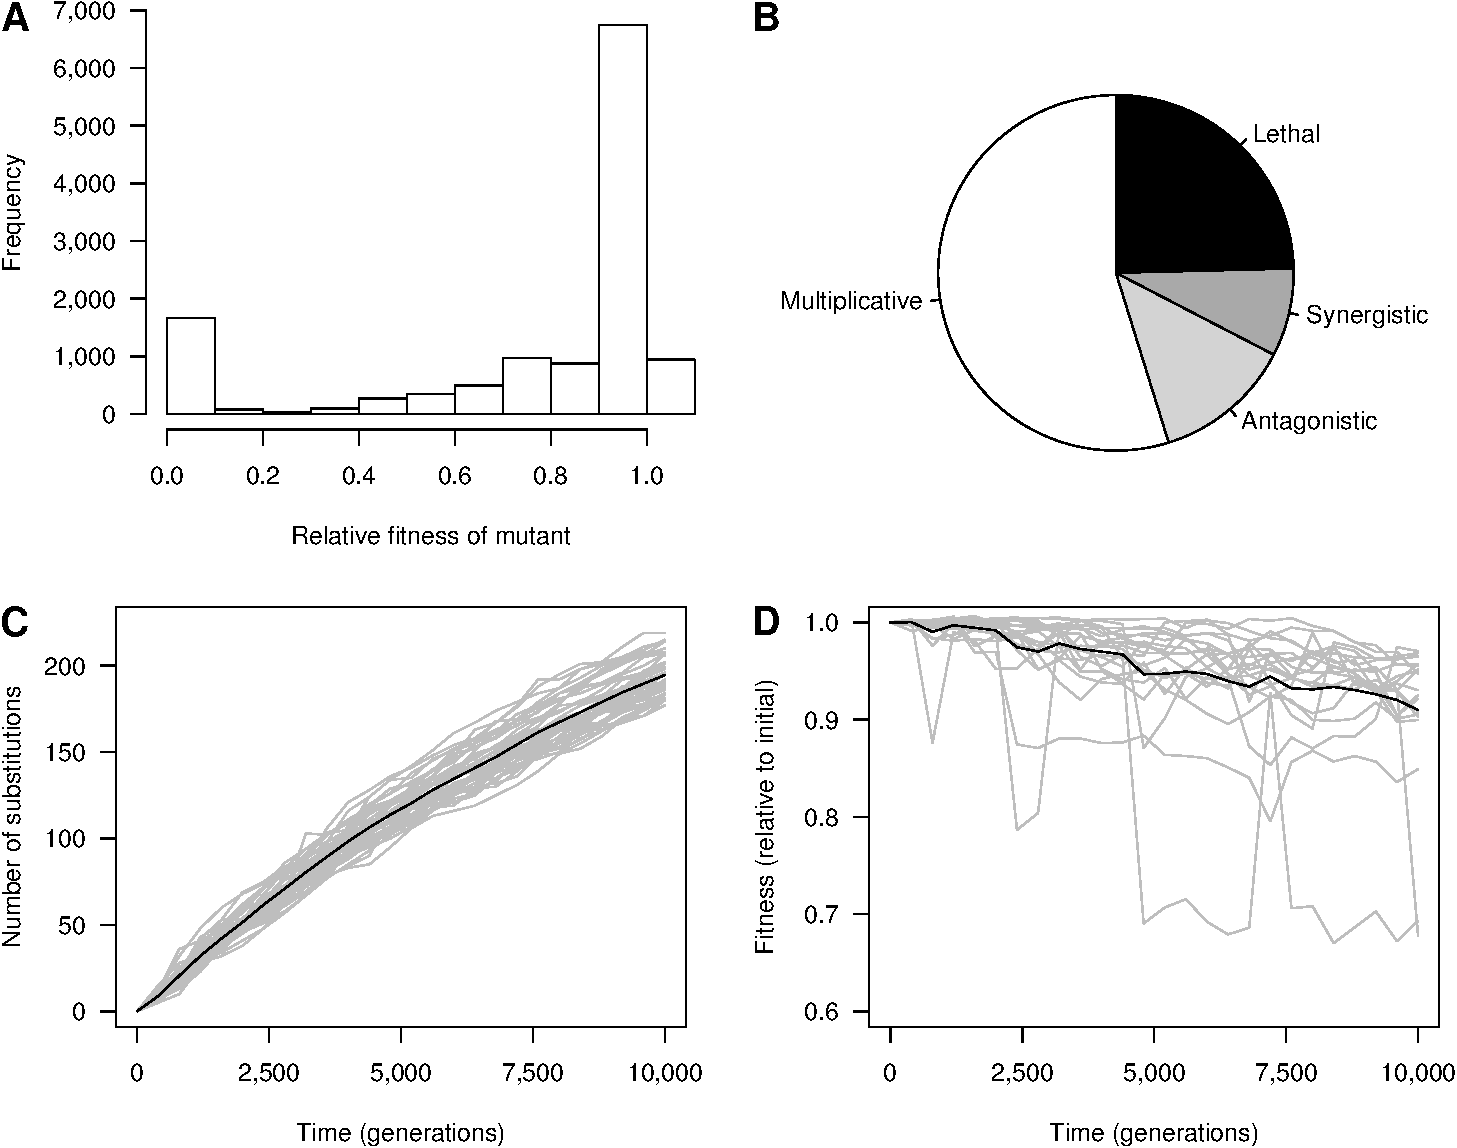
\includegraphics[width=5in]{avida.pdf}
\end{center}
\caption{
  (\textbf{A}) Fitness distribution of all possible single mutants
    of an evolved digital organism.
  (\textbf{B}) Proportions of epistasis types for an evolved digital organism.
  (\textbf{C}) Number of substitutions for each population through time
    (gray lines: individual replicates; black line: mean of replicates).
  (\textbf{D}) Fitness of hybrids between populations through time
    (gray lines: individual replicates; black line: mean of replicates).}
\label{avida}
\end{figure}



\subsection{Pairwise DMIs increased quadratically through time}

To count the number of pairwise DMIs between two species,
I separately counted the number of derived-ancestral
and derived-derived DMIs (Fig.~\ref{dmi-count-method}).
%
To find derived-ancestral DMIs, I first searched
for single derived alleles of each species
that were incompatible with the ancestral background
(e.g., allele~\emph{E} in Fig.~\ref{dmi-count-method}A, step~1).
%
I defined an allele as incompatible with the ancestral background
if the fitness of the ancestral genotype with that allele alone
was $<$~0.75 relative to the original ancestor.
%
To determine whether the incompatibility was due to a single ancestral allele
(thereby forming a derived-ancestral DMI), I searched for another
derived allele of the same species that rescued the incompatibility
(e.g., allele~\emph{C} in Fig.~\ref{dmi-count-method}A, steps~2 and 3).
%
I defined an incompatibly as rescued by another allele if the relative fitness
of the ancestral genotype with both alleles was $>$~0.99.
%
To ensure that the rescue allele was itself not involved in other DMIs,
I verified that its fitness in the ancestral background was also $>$~0.99.
%
I excluded testing rescue alleles that appeared after the derived allele
because in a derived-ancestral DMI a derived allele cannot be incompatible
with any current ancestral alleles (e.g., in Fig.~\ref{dm-model},
allele~\emph{C} cannot be incompatible with \emph{e}).
%
To find derived-derived DMIs, I searched for single derived alleles
from both species that were each compatible with the ancestral background
but together were incompatible (Fig.~\ref{dmi-count-method}B).
%
Using this two-part method, I counted the total number of pairwise DMIs
for each of the 20 replicate pairs of populations every 400 generations.



\begin{figure}[p]
\begin{center}
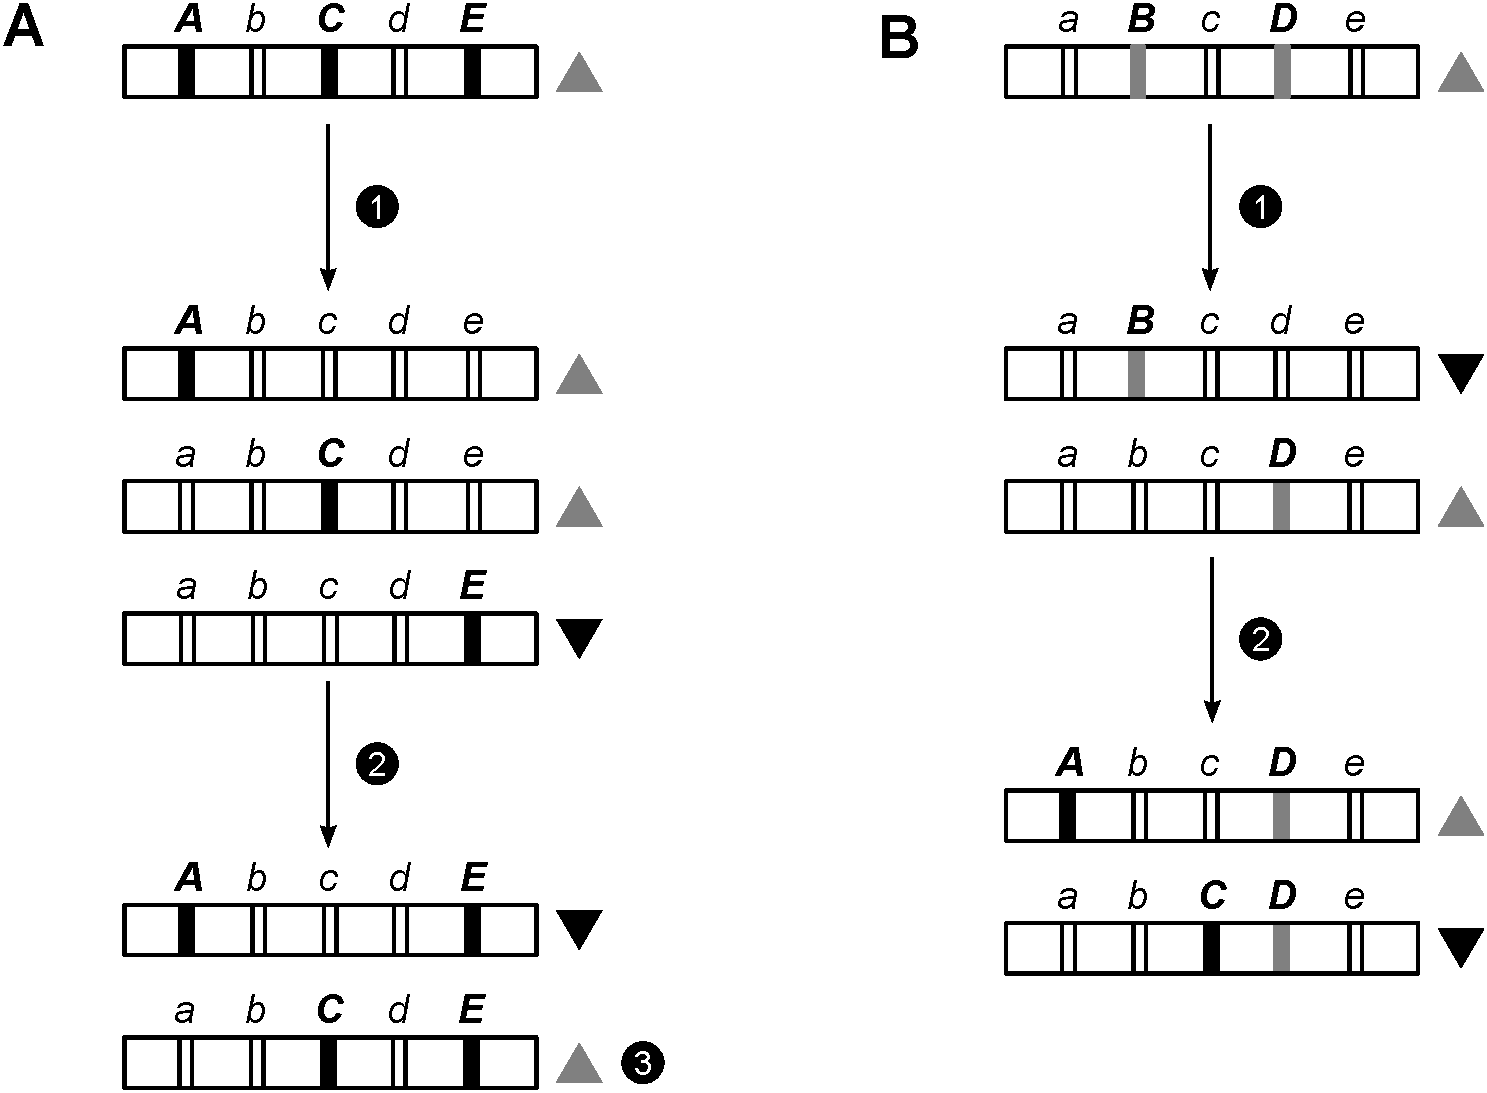
\includegraphics[width=5in]{dmi-count-method.pdf}
\end{center}
\caption{Illustration of the method for identifying
  (\textbf{A}) derived-ancestral
  and (\textbf{B}) derived-derived pairwise DMIs (see text).
  %
  (\textbf{A}) Step 1: I tested the individual fitness effect
  of each derived allele (black bars) of a species on the ancestral background.
  %
  Step 2: For each derived allele that
  was incompatible with the ancestral background
  (indicated by the black triangle pointing down),
  I tested the individual effect of the other derived alleles
  on that genetic background.
  %
  Step 3: If a second derived allele resulted in high fitness
  (indicated by the gray triangle pointing up),
  the ancestral allele at that second locus
  was incompatible with the original derived allele.
  %
  (\textbf{B}) Step 1: I tested the individual fitness effect
  of each derived allele (gray bars) of a species on the ancestral background.
  %
  Step 2: For each derived allele that
  was compatible with the ancestral background,
  I tested the individual effect of each derived allele
  (itself compatible with the ancestral background) of the other species.
  %
  Step 3: If the second allele lowered the fitness,
  then these two allele must be incompatible.}
\label{dmi-count-method}
\end{figure}



To determine whether a linear ($ax$) or a quadratic ($ax^{2} + bx$) model
best described the accumulation of pairwise DMIs through time,
I fit these two models to the whole dataset ($n = 520$)
and to each replicate individually (each $n = 26$).
%
Because there are no pairwise DMIs at the moment of geographic isolation,
the models do not have a constant term (i.e., the intercept is~0).
%
I estimated the parameters of each model using maximum likelihood
with a Gamma distribution for DMIs and compared the models using AIC
\citep{bol08}.
%
I found that the quadratic model explained the whole dataset better
than the linear model (Fig.~\ref{dmi-and-hybrids}A),
although there was considerable variation per replicate
(Fig.~\ref{fig:indiv-dmi}).
%
These results indicate that the overall accumulation of pairwise DMIs
was consistent with the snowball effect.



\begin{figure}
\begin{center}
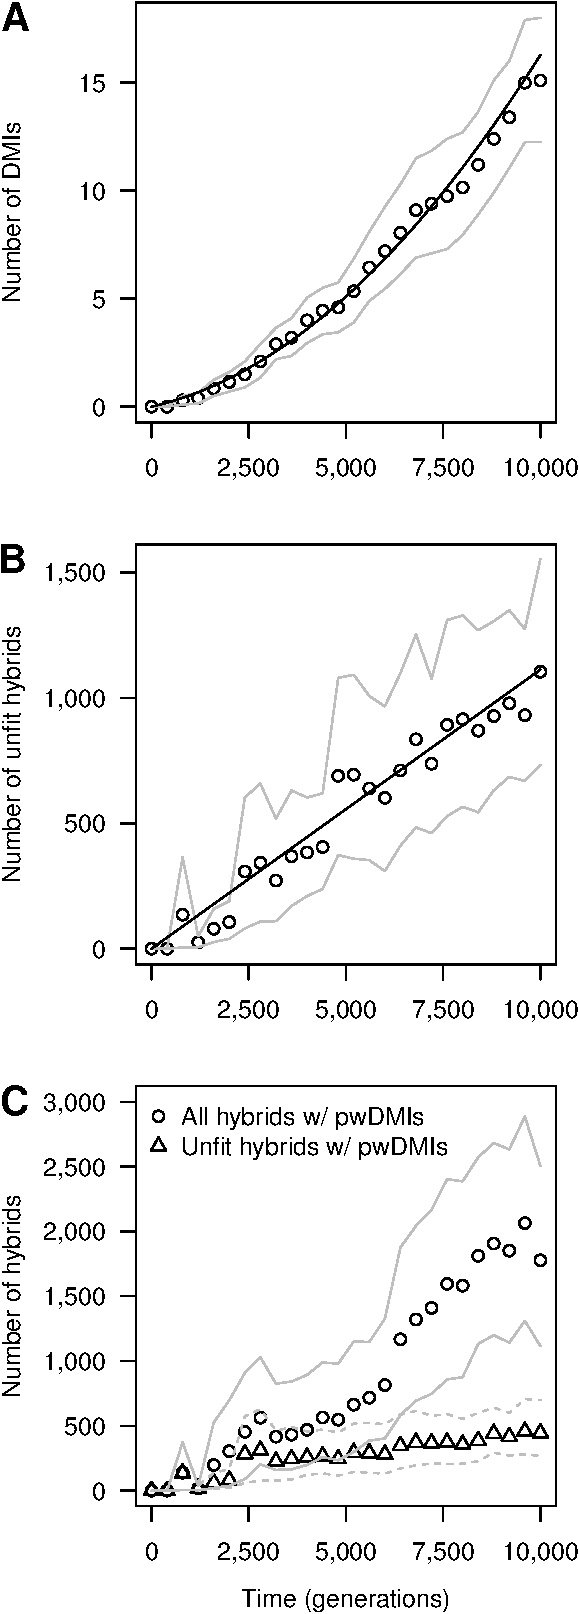
\includegraphics[height=6in]{dmi-and-hybrids.pdf}
\end{center}
\caption{
  (\textbf{A}) Mean number of pairwise DMIs through time.
  Each point represents the mean of 20 replicate runs.
  The black curve represents the quadratic model of the data
  with parameters estimated using maximum likelihood.
  The gray lines represent the bootstrap 95\% confidence intervals of the means.
  %
  (\textbf{B}) Mean number of unfit hybrids (out of 10,000)
  between populations through time.
  Each point represents the mean of 20 replicate runs.
  The black line represents the linear model of the data
  with parameters estimated using maximum likelihood.
  The gray lines represent the bootstrap 95\% confidence intervals of the means.
  %
  (\textbf{C}) Mean number of all hybrids () %find a circle symbol; $\medcirc$)
  and unfit hybrids ($\triangle$) (out of 10,000)
  with at least one pairwise DMI through time.
  Each point represents the mean of 20 replicate runs.
  The gray lines represent the bootstrap 95\%
  confidence intervals of the means.}
\label{dmi-and-hybrids}
\end{figure}



\begin{figure}
\begin{center}
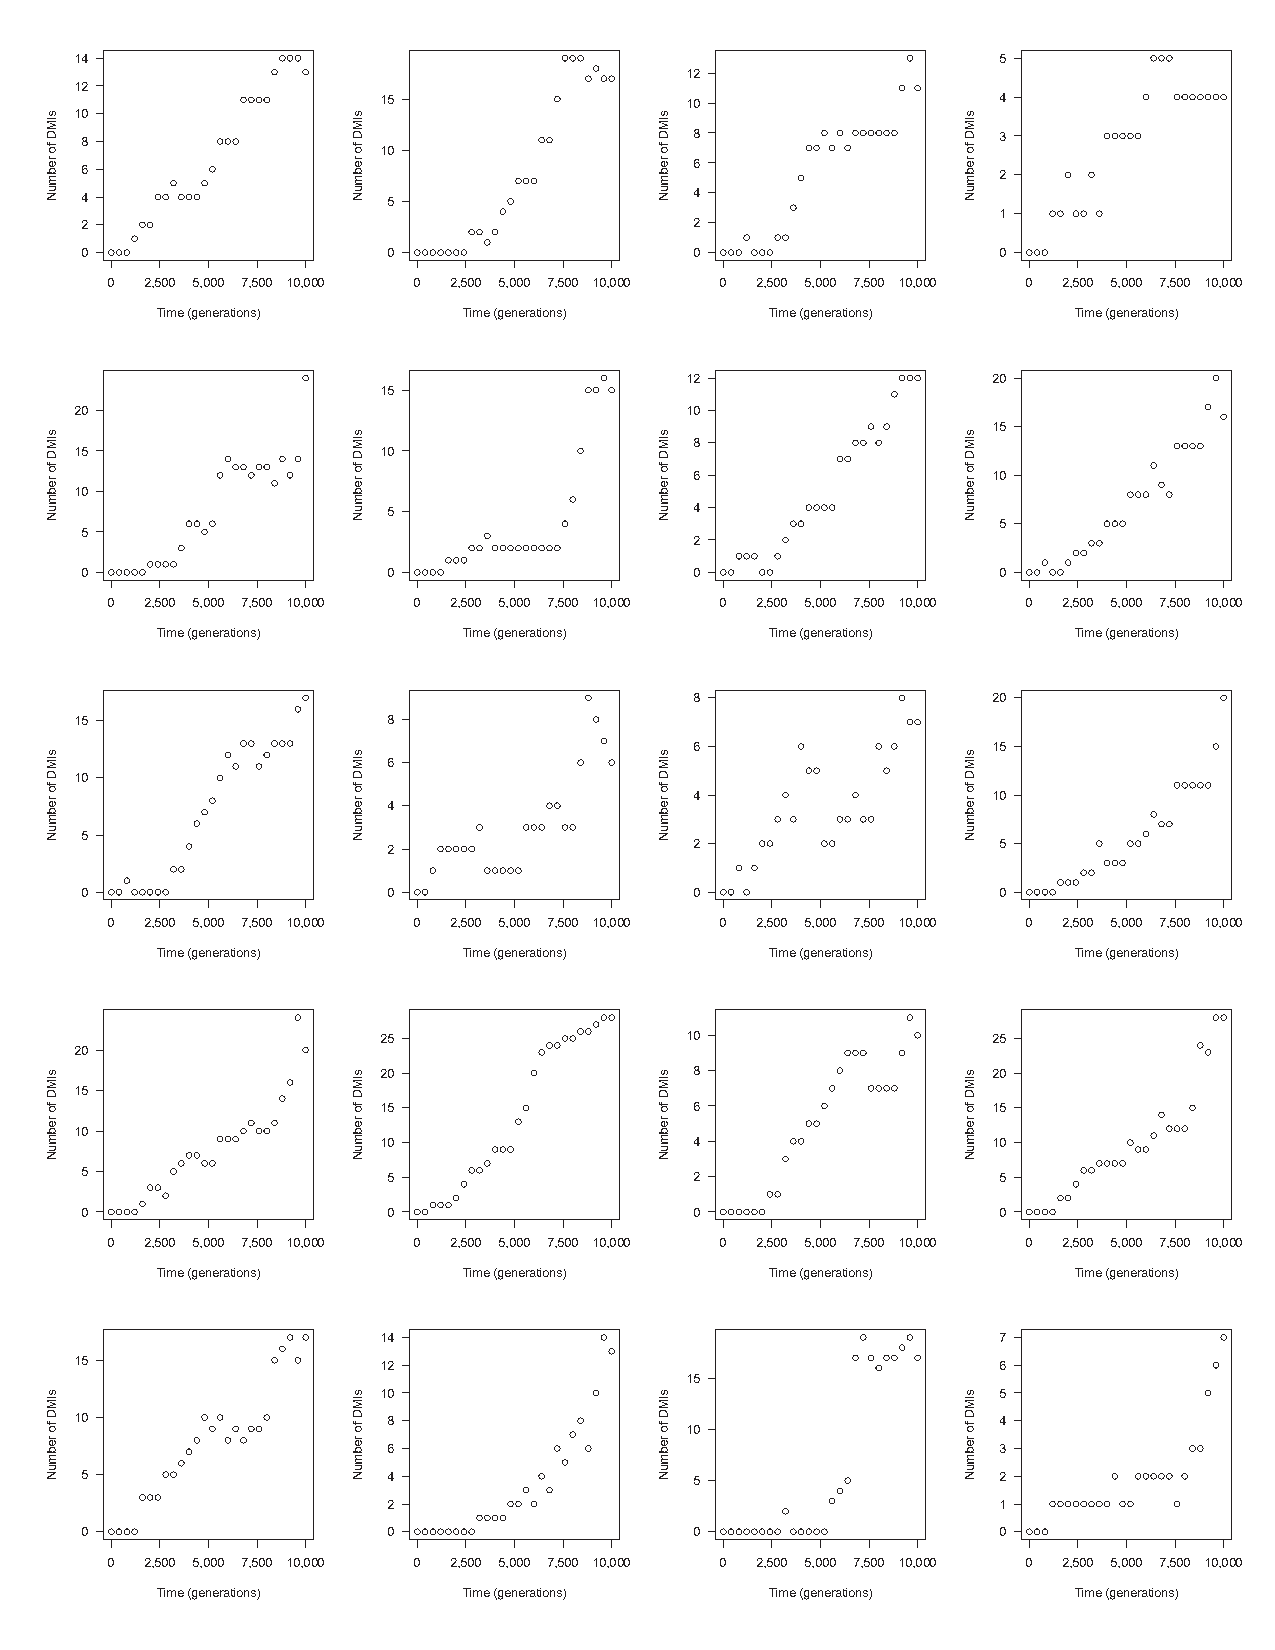
\includegraphics[width=0.9\linewidth]{dmi-counts-indiv-plots.pdf}
\end{center}
\caption{Number of pairwise DMIs through time
  between each replicate pair of populations.}
\label{fig:indiv-dmi}
\end{figure}



\subsection{Hybrid inviability increased linearly through time}

To measure hybrid inviability (i.e., number of unfit hybrids) through time,
I first created 10,000 hybrids between each replicate pair of species
every 400 generations.
%
Hybrids were created in the same way Avida recombines two genotypes:
two random but homologous regions of the parental genomes were exchanged.
%
Note that hybrids were created after the experiments were done,
using the populations I saved every 400 generations;
no hybridization between populations occurred during their evolution.
%
I then measured the fitness of each hybrid and counted the number
(out of 10,000) that had a relative fitness $<$~0.75.
%
I found that the overall number of unfit hybrids through time
increased linearly (Fig.~\ref{dmi-and-hybrids}B),
although there was considerable variation per replicate
(Fig.~\ref{fig:indiv-unfit-hybrids}).
%
These results are consistent with a missing snowball for hybrid inviability
and therefore suggest that the fitness effects of DMIs were not additive.



\begin{figure}
\begin{center}
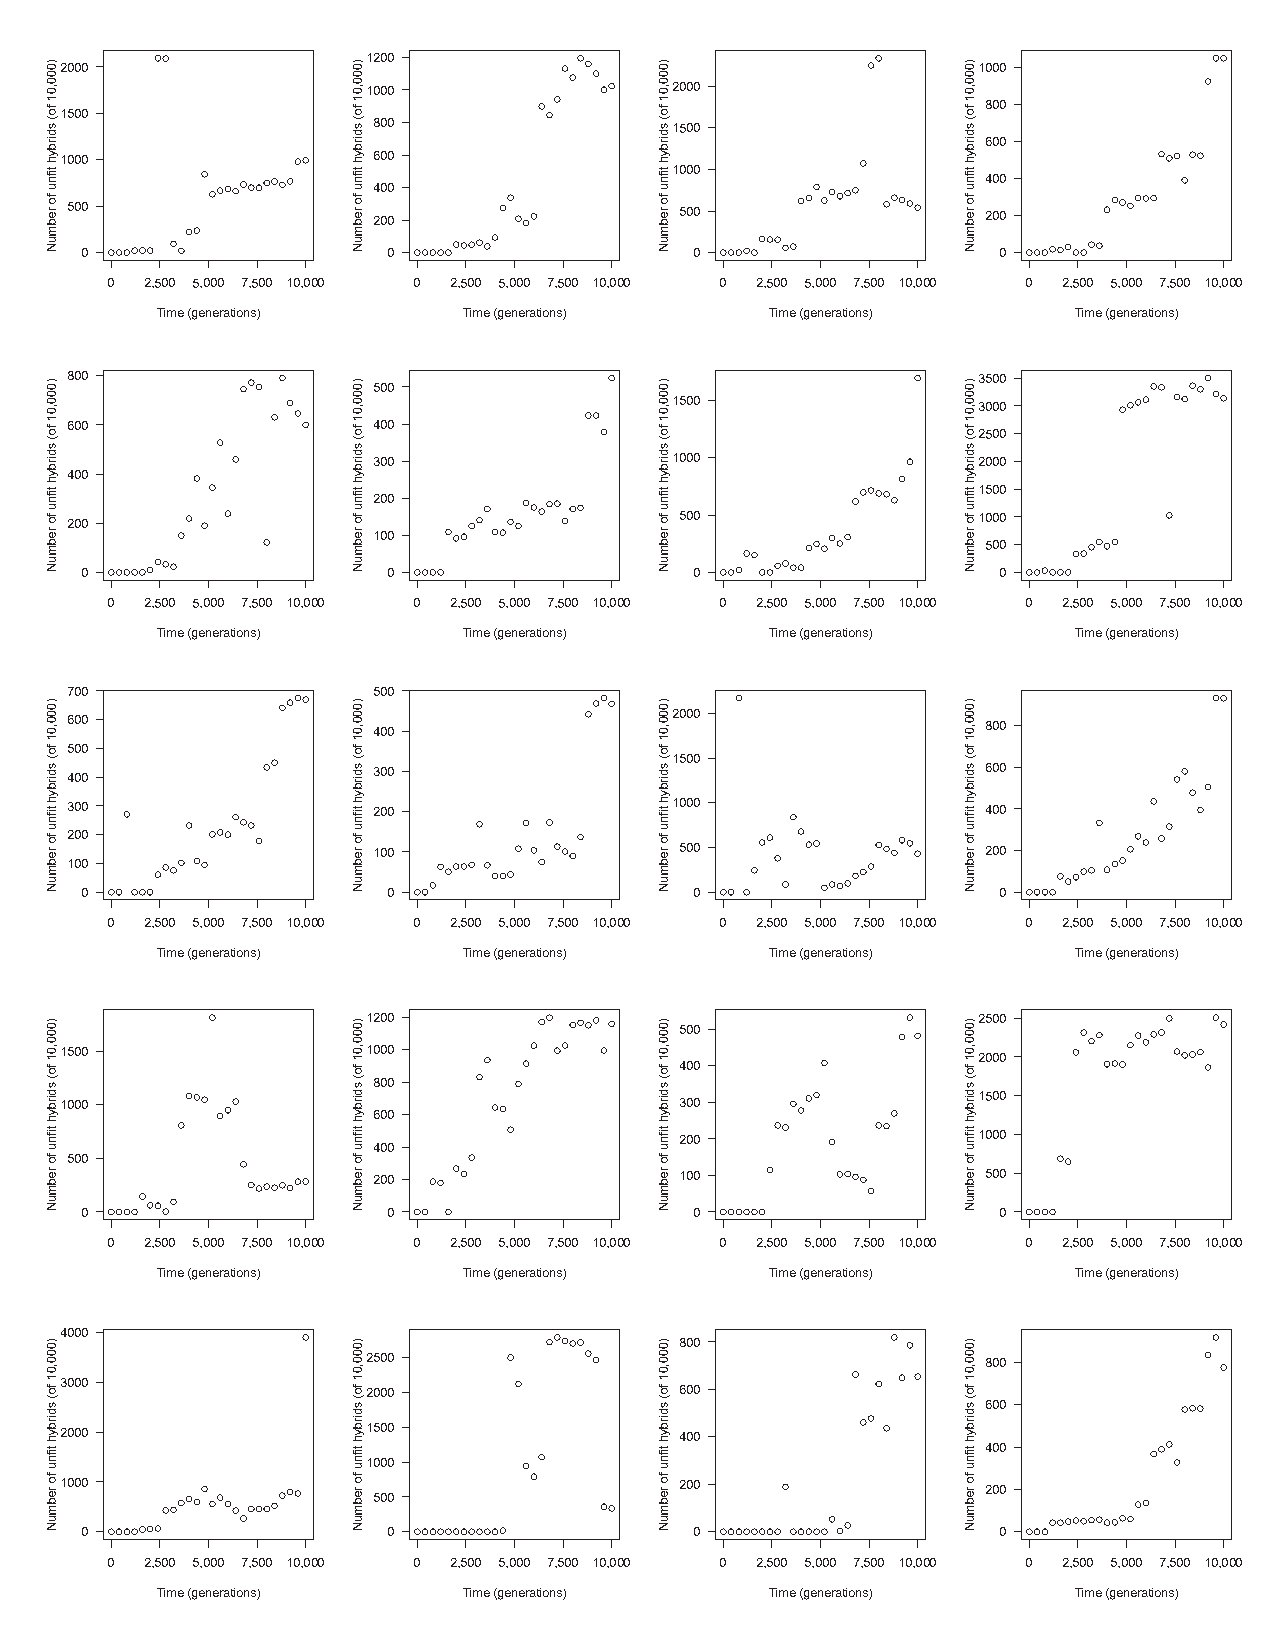
\includegraphics[width=0.9\linewidth]{unfit-hybrid-counts-indiv-plots.pdf}
\end{center}
\caption{Number of unfit hybrids (out of 10,000) through time
  between each replicate pair of populations.}
\label{fig:indiv-unfit-hybrids}
\end{figure}



\subsection{Secondary alleles rescue pairwise DMIs}

%Therefore, I found that in the same experiment
%the mean number of pairwise DMIs increased quadratically,
%while the mean hybrid inviability increased linearly.
Previous studies have found a linear increase
in hybrid inviability through time,
but conclusions that these results indicate the absence
of a snowball effect require that DMIs be additive.
%
If pairwise DMIs were additive, I would expect that hybrids
carrying at least one pairwise DMI be unfit
because a single pairwise DMI should reduce
the fitness of the carrier to $<$ 0.75.
%
I found, however, that not all hybrids
carrying at least one pairwise DMI were unfit
%(e.g., at the end of the runs, only $\sim$ 25\% of such hybrids were unfit)
(Fig. \ref{dmi-and-hybrids}C),
indicating that pairwise DMIs were not additive.
%may interact
%with other derived alleles that rescue the incompatibilities.
% I use 'rescue' to be able to connect it with Drosophila literature
%
One possible reason pairwise DMIs were not additive
is that other derived alleles present in the hybrid rescued pairwise DMIs
(i.e., the true incompatibility was greater than pairwise).
%
This hypothesis predicts that fit hybrids carrying a pairwise DMI
are more likely to carry a rescue allele than unfit hybrids.
%
To test this prediction,
I first identified all possible rescue alleles for all known pairwise DMIs
by searching for single derived alleles from either species
that rescued each known pairwise DMI.
%
Then, for hybrids carrying a pairwise DMI (at generation 10,000),
I calculated the proportion that also carried a rescue allele.
%
I found that 97\% of fit hybrids carried a rescue allele
compared to only 45\% of unfit hybrids.
%
This finding suggests that certain alleles rescued pairwise DMIs,
and this complex interaction could explain
why pairwise DMIs were not additive and therefore
why the mean hybrid inviability increased only linearly.


% Accumulation of DA vs DD DMIs

\subsection{Derived-ancestral DMIs occur as often as derived-derived}

Derived alleles have been predicted to be three times more likely
than ancestral alleles to be involved in pairwise DMIs \citep{orr95}.
%
To test this prediction, I counted the number of times
a derived allele appeared in a DMI
(once in a derived-ancestral DMI and twice in a derived-derived DMI)
and the number of times an ancestral allele appeared in a DMI
(once in a derived-ancestral DMI).
%
I made these counts at 10,000 generations for each pair of populations,
and I calculated the mean of the ratios between the number of derived alleles
and ancestral alleles found in all DMIs.
%
I found that derived alleles are 3.06 (2.41--3.79, 95\% bootstrap C.I.)
times more likely than ancestral alleles to appear in pairwise DMIs,
which experimentally supports the prediction.
%
However, the number of derived-ancestral and derived-derived DMIs
were comparable, suggesting that hybrid inviability due to
a missing dependent allele in the same species was just as likely due to
incompatible derived alleles between species.



\section{Discussion}

% I should say somewhere that the raw numbers of DMIs that form
% in digital organisms should not be taken to reflect biology
% (see review by Presgraves, 2010, AmNat for actual numbers)

% Example where genetics of hybrid sterility is "complex":
% Asymmetry and polymorphism of hybrid male sterility during the early stages of speciation in house mice

Although the mean accumulation of pairwise DMIs increased quadratically,
there was considerable variation in the pattern of accumulation
for individual species pairs (Fig.~S1).
%
There are at least three main possibilities for this variation.
%
First, the probability \emph{p} that two alleles are incompatible
may not be constant through time.
%
For example, a new derived allele may form multiple pairwise incompatibilities
with ancestral or derived alleles of the other population,
increasing the value of \emph{p} temporarily.
%
Second, as an evolving population navigates its neutral landscape,
a derived allele that once caused a DMI may later be replaced
by an allele that does not cause any DMIs.
%
Third, I used the majority-rule consensus sequence
of a population for our analyses,
but alleles in a consensus sequence are not necessarily fixed.
%
For example, an allele that was present in 51\% of the population
would appear in the consensus sequence,
but if that allele later decreases in frequency through drift
it could disappear from the consensus sequence.
%
If such an allele was involved in DMIs,
the estimated number of DMIs would change over time.
%
All of our population pairs underwent evolution
in the same environmental conditions,
yet showed variation in the accumulation of DMIs.
%
This variation suggests that in natural populations,
where environmental conditions between any taxa are rarely identical,
the accumulation of DMIs should also vary considerably.


Alleles that rescue hybrid fitness are not unique to digital organisms.
%
In \emph{Drosophila}, several `hybrid rescue mutations'
recover the viability or fertility
of hybrids between \emph{D. melanogaster} and closely-related species.
%
Note that the \emph{Drosophila} rescue alleles
were artificially selected mutations,
not derived alleles that were fixed in natural populations,
so the importance of rescue alleles in the wild is currently unknown.
%
Two hypotheses explain how rescue alleles
may interact with DMIs.
%
In the first hypothesis, rescue alleles
``suppress the effects of the loci causing hybrid problems'' \citep{coy04}.
%
In this case, rescue alleles may be products of genetic redundancy,
which itself may have evolved as a `buffering mechanism'
against deleterious mutations \citep{wag99,ele06}.
%
For example, a genotype that gains a new allele performing
overlapping functions with another allele at a different locus
will be more robust to deleterious mutations that affect those functions.
%
Although I do not know whether rescue alleles in our system are redundant,
studies have shown that sexual, complex digital organisms
with high mutation rates exhibit mutational robustness \citep{len99,wil01,mis06},
which can evolve by genetic redundancy \citep{ele07}.
%
According to the second hypothesis, rescue alleles
``represent mutations at the actual loci
that cause the death or sterility of hybrids'' \citep{coy04}.
%
This hypothesis implies that hybrid incompatibilities
thought to involve only two alleles actually involve three or more,
as in the case with the hybrid rescue mutation
\emph{Hmr} in \emph{Drosophila} \citep{bar00,orr00}.
%
% EXPLAIN FOLLOWING SENTENCE BETTER (Emily Weigel)
Similarly, if this hypothesis applies
to the rescue alleles I discovered in digital organisms,
then any presumed `pairwise' DMI that was rescued by a third allele
was, in fact, a three-way DMI.
%
Therefore, rescue alleles may provide evidence that complex DMIs,
which are exceptionally difficult to identify in biological organisms,
are common in biological and digital organisms.
% For the above explanation, I'm going to want to invoke
% Maheshwari & Barbash, 2012, which talk about DA DMIs
% possibly being three-way incompatibilities


%Our study reconciles the prediction of a snowball effect
%of the Dob\-zhan\-sky-Mul\-ler model of postzygotic isolation
%with the empirical observation of a ``missing snowball.''
%
In summary, using an artificial life software
I found that pairwise DMIs accumulate quadratically through time,
supporting the snowball effect
and the Dob\-zhan\-sky-Mul\-ler model of postzygotic isolation.
%
In addition, I discovered that the number of derived-ancestral 
and derived-derived DMIs are similar,
suggesting that hybrid inviability due to
a missing allele in the same species
were just as likely due to
incompatible derived alleles between species.
%
When I used the strength of postzygotic isolation
as a proxy for the number of DMIs,
I found a linear, rather than quadratic,
relationship with divergence time.
%
This discrepancy was at least partially caused by rescue alleles,
which I found recovered the negative effects of DMIs in hybrids,
disrupting the pattern of quadratic increase of DMIs.
%
Our findings indicate that pairwise DMIs are insufficient
to account for the complexity of epistatic interactions
among alleles within and between species.
%
Thus, our results highlight the importance of complex interactions
in the genetics of reproductive isolation.

%% Stronger concluding paragraph -- Emily

%I started with how reproductive isolation evolves,
%how has this study helped answer that question?

%RI can evolve through drift



%% FINAL PARAGRAPH
%The effect of selection on the accumulation of DMIs, however,
%remains to be experimentally tested,
%although mathematical models have considered selection \citep{unc09}.
%
%Another interesting thing is
%the effect of gene flow on the accumulation of DMIs,
%providing a genetic mechanism by which isolation is slowed.
%
%Other models have examined the effect of gene flow
%during divergence \citep{kon03}.
%
%Artificial life offers opportunity to study these things empirically.


% Maybe boil down the above to 1 or 2 sentence
% and add to the previous paragraph,
% which itself may be boiled down so it's not too long


% PUT IN METHODS AT THE END
%In Avida, digital organisms consist of a sequence of instructions (or `genome')
%that encodes their ability to replicate and perform computational functions.
%
%Sexual reproduction between two organisms
%exchanges a random but homologous region of their genomes,
%then places the recombinants back into the population.
%
%Organisms are rewarded with a higher replication rate if they evolve
%the ability to perform computational functions,
%which require specific but not unique sequences of instructions.
%
%Variation in the efficiency of replication and in the ability
%to perform functions arises via recombination and mutation.
%
%Because faster replicators in a finite population leave
%more copies of themselves, digital organisms evolve via natural selection
%and genetic drift (i.e., evolution is not simulated).
%
%Fitness, an estimate of an organism's reproductive rate,
%is measured as the amount of rewards obtained divided
%by the number of steps required to replicate.
%
%Although there are many parameters in Avida
%that can be configured (e.g., mutation rate),
%evolutionary processes like natural selection
%and epistasis occur spontaneously.
%
%With Avida, I can
%observe millions of generations of evolution in real-time,
%replicate experiments with identical starting conditions,
%easily manipulate genomes, and
%accurately record measurements
%like fitness and events like mutations.

\section{Methods}

\subsection{Experimental configuration}

The environment was configured to reward the nine default tasks
and 68 additional three-input tasks.
%
All tasks were set to provide a resource value of 1 in an additive fashion;
resources were unlimited.
%
The maximum population size was set to 100 organisms,
and the length of each organism's genome was fixed at 500 instructions.
%
The `copy' mutation probability---the probability that an organism
would copy a random instruction rather than its own to its offspring---%
was set to 0.1 per genome per generation
(all other mutation probabilities were set to 0.0).
%
Mutation to the `h-copy' instruction was turned off to prevent
organisms from using up their genomic space with h-copy instructions
(rather than task-related instructions), which was a common way
to improve their replication efficiency in preliminary runs.
%
Offspring were configured to replace a random organism in the population.



\subsection{Statistics}

Statistical analyses were carried out using R (ver. 2.15.1) \citep{r13}.
%
To perform the AIC analyses, I used the bbmle package \citep{bol08}
and the mle2 function with the `Nelder-Mead' optimization method.
%




\section{Acknowledgments}

I thank A. P. Dreyer, E. M. Swanson, R. E. Lenski, J. W. Boughman,
E. Weigel, E. Dittmar, L. J. Harmon, and D. R. Matute
for helpful comments on the manuscript.
%
This material is based in part upon work supported
by the National Science Foundation under Cooperative Agreement No. DBI-0939454.
Any opinions, findings, and conclusions or recommendations
expressed in this material are those of the author
and do not necessarily reflect the views of the National Science Foundation.



\end{doublespace}

\bibliographystyle{apalike}
\bibliography{snowball}
